\begin{examplebox}
  \textbf{\textcolor{CExample}{例1｜二次函数：横坐标压缩为 $1/3$（基础）}}
  \textbf{题目：} 将 $y=x^2$ 图像上所有点的横坐标变为原来的 $1/3$，纵坐标不变。求新函数解析式。

  \textbf{解题：} 横坐标要\textbf{除以 $3$}，所以解析式中要把 $x$ \textbf{乘 $3$}：
  \[
    \boxed{\ y=f(3x)=(3x)^2=9x^2\ }.
  \]
  \textbf{用数字核对：} 原图像经过 $(2,4)$，新图像就经过 $(2/3,4)$；把 $x=2/3$ 代入 $y=9x^2$，确实得到 $4$。
  \begin{center}
  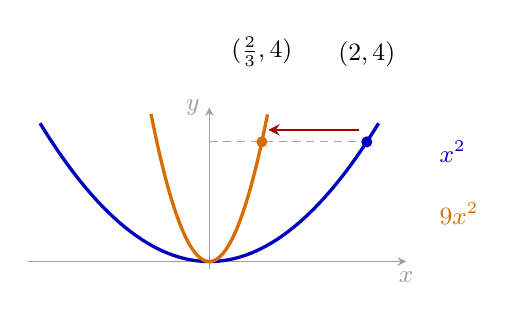
\begin{tikzpicture}[x=1.0cm,y=0.38cm,>=stealth,every node/.style={font=\small}]
    \draw[->,gray!75] (-2.3,0)--(2.5,0) node[below] {$x$};
    \draw[->,gray!75] (0,-0.25)--(0,5.15) node[left] {$y$};
    \draw[very thick,blue!75!black,domain=-2.15:2.15,samples=70] plot (\x,{\x*\x});
    \draw[very thick,orange!85!black,domain=-0.74:0.74,samples=70] plot (\x,{9*\x*\x});
    \draw[densely dashed,gray!70] (0,4)--(2,4);
    \fill[blue!75!black] (2,4) circle (2pt);
    \fill[orange!85!black] (0.667,4) circle (2pt);
    \draw[->,thick,red!65!black] (1.9,4.4)--(0.75,4.4);
    \node[blue!75!black,above right] at (2.8,3.0) {$x^2$};
    \node[orange!85!black,right] at (2.8,1.6) {$9x^2$};
    \node[above] at (2,6.2) {$(2,4)$};
    \node[above] at (.667,6.2) {$(\frac23,4)$};
  \end{tikzpicture}

  \end{center}
  \textbf{考试快法：} 看见“横坐标缩为 $1/3$”，立刻把式子里的 $x$ 换成 $3x$。

  \medskip
  \textbf{\textcolor{CExample}{例2｜对数函数：横坐标扩大到 $2$ 倍（变形）}}
  \textbf{题目：} 将 $y=\ln x$ 的图像横向拉宽 $2$ 倍，求新函数解析式，并指出定义域。

  \textbf{解题：} 横坐标\textbf{乘 $2$}，括号里的 $x$ 就\textbf{除以 $2$}：
  \[
    \boxed{\ y=\ln\!\left(\frac{x}{2}\right),\quad x>0\ }.
  \]
  \textbf{用数字核对：} 原函数的点 $(1,0)$ 移到 $(2,0)$；原来 $(2,\ln 2)$ 移到 $(4,\ln2)$。\textbf{对数的输入必须大于 $0$}，所以新函数仍要求 $x>0$。
  \begin{center}
  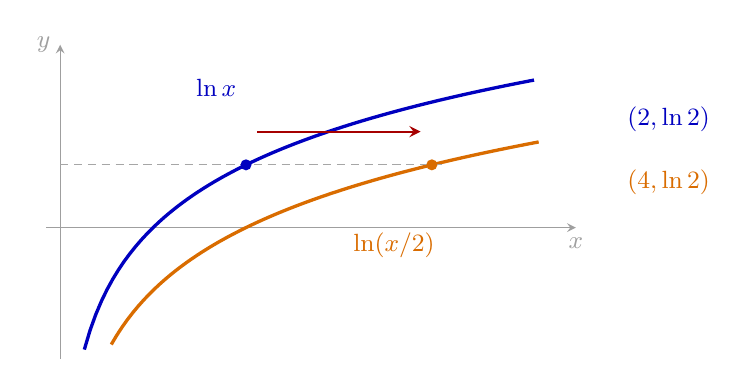
\begin{tikzpicture}[x=1.18cm,y=1.15cm,>=stealth,every node/.style={font=\small}]
    \draw[->,gray!75] (0,-1.45)--(0,2.02) node[left] {$y$};
    \draw[->,gray!75] (-0.15,0)--(5.55,0) node[below] {$x$};
    \draw[very thick,blue!75!black,domain=0.26:5.1,samples=80] plot (\x,{ln(\x)});
    \draw[very thick,orange!85!black,domain=0.55:5.15,samples=80] plot (\x,{ln(\x/2)});
    \draw[densely dashed,gray!70] (0,{ln(2)})--(4.15,{ln(2)});
    \fill[blue!75!black] (2,{ln(2)}) circle (2pt);
    \fill[orange!85!black] (4,{ln(2)}) circle (2pt);
    \draw[->,thick,red!65!black] (2.12,1.06)--(3.88,1.06);
    \node[blue!75!black,above left] at (2,1.34) {$\ln x$};
    \node[orange!85!black,below right] at (3.05,0.05) {$\ln(x/2)$};
    \node[anchor=west,blue!75!black] at (6,1.2) {$(2,\ln2)$};
    \node[anchor=west,orange!85!black] at (6,.5) {$(4,\ln2)$};
  \end{tikzpicture}

  \end{center}
  \textbf{考试快法：} 想让图像变宽，就要\textbf{让函数内部变化得更慢}，因此用 $x/2$ 而不是 $2x$。

  \medskip
  \textbf{\textcolor{CExample}{例3｜三角函数：先横向压缩，再向上平移（综合）}}
  \textbf{题目：} 将 $y=\sin x$ 的图像先横向压成原来的 $1/2$，再向上平移 $1$ 个单位，求新解析式。

  \textbf{解题：} 第一步\textbf{横坐标减半}：$y=\sin(2x)$；第二步\textbf{高度增加 $1$}：
  \[
     \boxed{\ y=\sin(2x)+1\ }.
  \]
  \textbf{用数字核对：} 原来 $(\pi/2,1)$，压缩后是 $(\pi/4,1)$，再上移成 $(\pi/4,2)$；代入最终式子，$\sin(\pi/2)+1=2$。
  \begin{center}
  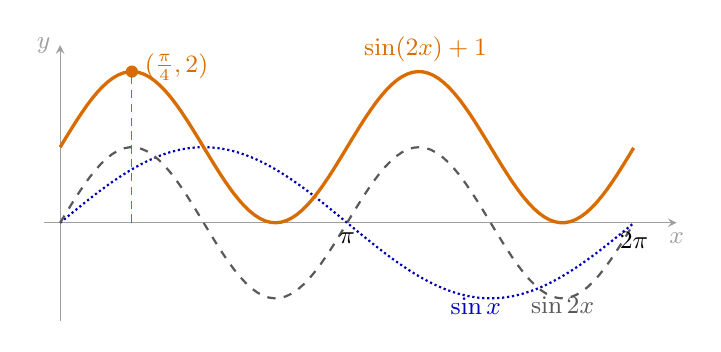
\begin{tikzpicture}[x=1.16cm,y=0.96cm,>=stealth,every node/.style={font=\small}]
    \draw[->,gray!75] (-0.18,0)--(6.75,0) node[below] {$x$};
    \draw[->,gray!75] (0,-1.3)--(0,2.35) node[left] {$y$};
    \draw[blue!70!black,densely dotted,thick,domain=0:6.28,samples=100] plot (\x,{sin(deg(\x))});
    \draw[gray!70!black,dashed,thick,domain=0:6.28,samples=100] plot (\x,{sin(deg(2*\x))});
    \draw[orange!85!black,very thick,domain=0:6.28,samples=110] plot (\x,{1+sin(deg(2*\x))});
    \fill[orange!85!black] (0.7854,2) circle (2.2pt);
    \draw[densely dashed,orange!75!black] (0.7854,0)--(0.7854,2);
    \node[right,orange!85!black] at (0.82,2.06) {$(\frac\pi4,2)$};
    \node[blue!75!black] at (4.55,-1.1) {$\sin x$};
    \node[gray!70!black,below] at (5.5,-0.85) {$\sin 2x$};
    \node[orange!85!black,above] at (4.0,2.0) {$\sin(2x)+1$};
    \node[below] at (3.1416,0) {$\pi$};
    \node[below] at (6.2832,0) {$2\pi$};
  \end{tikzpicture}

  \end{center}
  \textbf{特别提醒：} 本例的\textbf{横向伸缩}与\textbf{向上平移}交换顺序，结果仍相同；但如果改成\textbf{向右平移}，一般不能随意交换顺序（见易错点四）。
\end{examplebox}
